\section{Algorithm-level Designs}
\subsection{Training in Clean Pipeline}
\textbf{Multi-Shot Interactive AR Training.}\label{sec:interactive_training}$\;$

The AR objective and efficient teacher-forcing layout are described in \S~\ref{sec:sp_training}; here we focus on the algorithmic interface enabled by chunk-level generation. We employ Wan2.2-TI2V-5B~\cite{wan} as our base model.
We treat each temporal latent chunk $\mathbf{Z}_i$ as an editable generation unit and bind it to an individual text prompt $\mathbf{T}_i$.
Cross-attention is factorized per chunk as $\text{CrossAttn}(\mathbf{Z}_i, \mathbf{T}_i)$, rather than conditioning the whole video on a single global prompt.
This decoupling lets different shots carry different prompts, supports prompt switches at chunk boundaries, and preserves previously generated history when the user edits future chunks.



\textbf{Few-step Distillation.} \label{sec:dmd}$\;$
Our few-step distillation framework is derived from LongLive, but with several important simplifications. 
First, because the AR-trained model already supports long-video generation, we avoid the original multi-stage strategy with ODE initialization, short-video DMD, and streaming long-tuning DMD.
We instead perform one-stage DMD distillation on top of the AR-trained model, yielding a cleaner formulation without separate initialization or progressive long-tuning stages. 
Second, we do not fully fine-tune the DiT backbone; instead, we optimize LoRA modules only during the entire distillation process. This choice leads to more stable optimization and makes the resulting few-step capability easily transferable to any Wan2.2-TI2V-5B-based AR model. 
Specifically, we initialize the student, critic, and teacher from the original Wan2.2-TI2V-5B model. Similar to LCM-LoRA~\cite{luo2023lcm}, we find that the trained LoRA can be directly plugged into the AR model to reduce inference steps without further tuning.
In the end, the distilled model reduces generation to two steps, while preserving the long-video generation ability of the original framework.
We discuss the differences between our strategy and straightforward DMD fine-tuning in Appendix (\S~\ref{ap:dmd_comparison}).

\begin{figure}[t]
\centerline{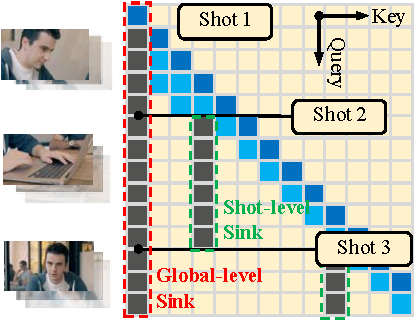
\includegraphics[width=0.72\columnwidth]{figs/shot-level-sink.pdf}}
\caption{\textbf{Multi-shot Attention Sink for streaming multi-shot inference.}}
\label{fig:shot-level-sink}
\end{figure}
\subsection{Inference with Multi-Shot Attention Sink}\label{sec:multi_shot_attention_sink}

To deploy our model for multi-shot streaming, we adopt sliding-window self-attention with KV caching to cap the per-step compute footprint at $\mathcal{O}(W\!\cdot\! L_c)$, where $W$ is the attention-window length in chunks and $L_c$ is the token length of each chunk. 
However, naively discarding tokens outside the window causes appearance drift. While standard attention sinks~\cite{xiao2023efficient} mitigate this by pinning the first few video frames, they fail in multi-shot settings: a single global sink cannot preserve \textit{intra-shot} coherence, while a moving shot-level sink loses \textit{global} identity.

\begin{table}[t]
\centering
\caption{AR training efficiency of LongLive-2.0. We compare end-to-end iteration time (seconds); red subscripts denote speedup over BF16+SP.}
\label{tab:wan22_ffn1_nvfp4}
\scriptsize
\resizebox{\linewidth}{!}{
\begin{tabular}{c c c c c}
\toprule
\rowcolor{gray!12}
\shortstack{\textbf{Input}\\\textbf{Length}} &
\shortstack{\textbf{BF16}\\\textbf{w/o SP}} &
\shortstack{\textbf{BF16}\\\textbf{w/ SP}} &
\shortstack{\textbf{BF16}\\\textbf{Balanced SP}} &
\shortstack{\textbf{NVFP4}\\\textbf{Balanced SP}} \\
\midrule
16s & 75.3 & 52.2 & 45.8 &
$\mathbf{40.1}_{\textcolor{DeepRed}{\scriptstyle \mathbf{1.3}\times}}$ \\
32s & 202.7 & 162.7 & 136.8 &
$\mathbf{119.3}_{\textcolor{DeepRed}{\scriptstyle \mathbf{1.4}\times}}$ \\
64s & OOM & 1372.9 & 1196.5 &
$\mathbf{639.5}_{\textcolor{DeepRed}{\scriptstyle \mathbf{2.1}\times}}$ \\
\bottomrule
\end{tabular}}
\end{table}
\begin{table}[t]
\centering
\caption{Progressively quantizing the generator, real-score, and fake-score models in DMD training. We report peak per-GPU memory.}
\label{tab:dmd_nvfp4_scaling}
\scriptsize
\setlength{\tabcolsep}{2.8pt}
\renewcommand{\arraystretch}{1.12}
\resizebox{\linewidth}{!}{%
\begin{tabular}{l l l r c}
\toprule
\rowcolor{gray!12}
\textbf{Generator} &
\textbf{Real} &
\textbf{Fake} &
\shortstack{\textbf{Peak Memory}} &
\shortstack{\textbf{Ratio} $\downarrow$} \\
\midrule
BF16 & BF16 & BF16 & 70.5 GB & - \\
\textbf{NVFP4} & BF16 & BF16 & 63.3 GB & 0.90$\times$ \\
\textbf{NVFP4}+LoRA & \textbf{NVFP4} & BF16 & 57.2 GB & 0.81$\times$ \\
\cdashline{1-5}
\textbf{NVFP4}+LoRA &
\textbf{NVFP4} &
\textbf{NVFP4}+LoRA &
\textbf{49.0 GB} &
\textcolor{DeepRed}{\textbf{0.69$\times$}} \\
\bottomrule
\end{tabular}%
}
\end{table}

\textbf{Multi-Shot Attention Sink.} $\;$
To resolve this, we introduce a multi-shot attention sink with two cooperating anchor sets (Figure~\ref{fig:shot-level-sink}): \textit{Global Sink} ($\mathcal{A}_{g}$): the first $S_g$ frames of the video, permanently fixed to preserve global identity. \textit{Shot-Level Sink} ($\mathcal{A}_{s}$): the first $S_s$ frames of the \emph{current} shot, re-bound at every scene cut to maintain local temporal coherence.


At any chunk generation step $t$, the effective key/value set is $\mathcal{K}_{\text{eff}}(t) = \mathcal{A}_{g} \cup \mathcal{A}_{s} \cup \mathrm{KV}_{[t-W, t)}$, with overlapping tokens deduplicated. $\mathcal{A}_{s}$ incurs zero memory overhead: it is tracked merely via two scalar pointers (\textsc{start}, \textsc{len}). It is virtually prepended to the sliding window only after the window rolls past it, avoiding data copying.


\textbf{Interaction with Chunk-wise Prompting.} $\;$
Crucially, this mechanism integrates seamlessly with our chunk-wise interactive prompting (\S~\ref{sec:interactive_training}). A prompt switch $p_{k}\!\to\!p'_{k}$ inherently defines a scene cut. This simply triggers the local re-binding of $\mathcal{A}_{s}$ to the new chunk and re-initializes the subsequent cross-attention cache, leaving the global sink $\mathcal{A}_{g}$ and preceding history untouched. This strict decoupling enables minute-scale interactive generation without redundant recomputation.